%%%%%%%%%%%%%%%%%%%%%%%%%%%%%%%%%%%%%%%%%
% Developer CV
% LaTeX Template
% Version 1.1 (February 24, 2025)
%
% This template originates from:
% https://www.LaTeXTemplates.com
%
% Authors:
% Jan Vorisek (jan@vorisek.me)
% Based on a template by Jan Küster (info@jankuester.com)
% Modified for LaTeX Templates by Vel (vel@LaTeXTemplates.com)
%
% License:
% The MIT License (see included LICENSE file)
%
%%%%%%%%%%%%%%%%%%%%%%%%%%%%%%%%%%%%%%%%%

%----------------------------------------------------------------------------------------
%	PACKAGES AND OTHER DOCUMENT CONFIGURATIONS
%----------------------------------------------------------------------------------------

\documentclass[10pt]{../developercv} % Default font size, values from 8-12pt are recommended
\usepackage{graphicx}
\graphicspath{{../images/}} % Path to the images folder

%----------------------------------------------------------------------------------------

\begin{document}

%----------------------------------------------------------------------------------------
%	TITLE AND CONTACT INFORMATION
%----------------------------------------------------------------------------------------

\begin{minipage}[t]{0.47\textwidth} % Left column with your name and title, change the width as needed
	\vspace{-\baselineskip} % Required for vertically aligning minipages

	% If your name is very short: use just one of the lines below
	% If your name is very long: reduce the font size or make the current column wider (and reduce the others proportionately)
	\colorbox{black}{{\HUGE\textcolor{white}{\textbf{\MakeUppercase{Stefan}}}}} % First name

	\colorbox{black}{{\HUGE\textcolor{white}{\textbf{\MakeUppercase{Schärmeli}}}}} % Last name

	\vspace{6pt} % Vertical whitespace

	{\LARGE Fullstack DevOps Engineer} % Career or current job title
\end{minipage}
\hfill % Automatic horizontal whitespace
\begin{minipage}[t]{0.25\textwidth} % Center column with the first column of icons
	\vspace{-\baselineskip} % Required for vertically aligning minipages

	% The first parameter is the FontAwesome icon name, the second is the box size and the third is the text
	% Other icons can be found by referring to fontawesome5.pdf (supplied with the template) and using the word after \fa in the command for the icon you want
	\icon{MapMarker}{12}{Bern}\\
	\icon{BirthdayCake}{12}{02-06-1983}\\
	\icon{Ring}{12}{single}\\
	\icon{Phone}{12}{+41 76 368 66 16}
\end{minipage}
\hfill % Automatic horizontal whitespace
\begin{minipage}[t]{0.23\textwidth} % Center column with the first column of icons
	\vspace{-\baselineskip} % Required for vertically aligning minipages
	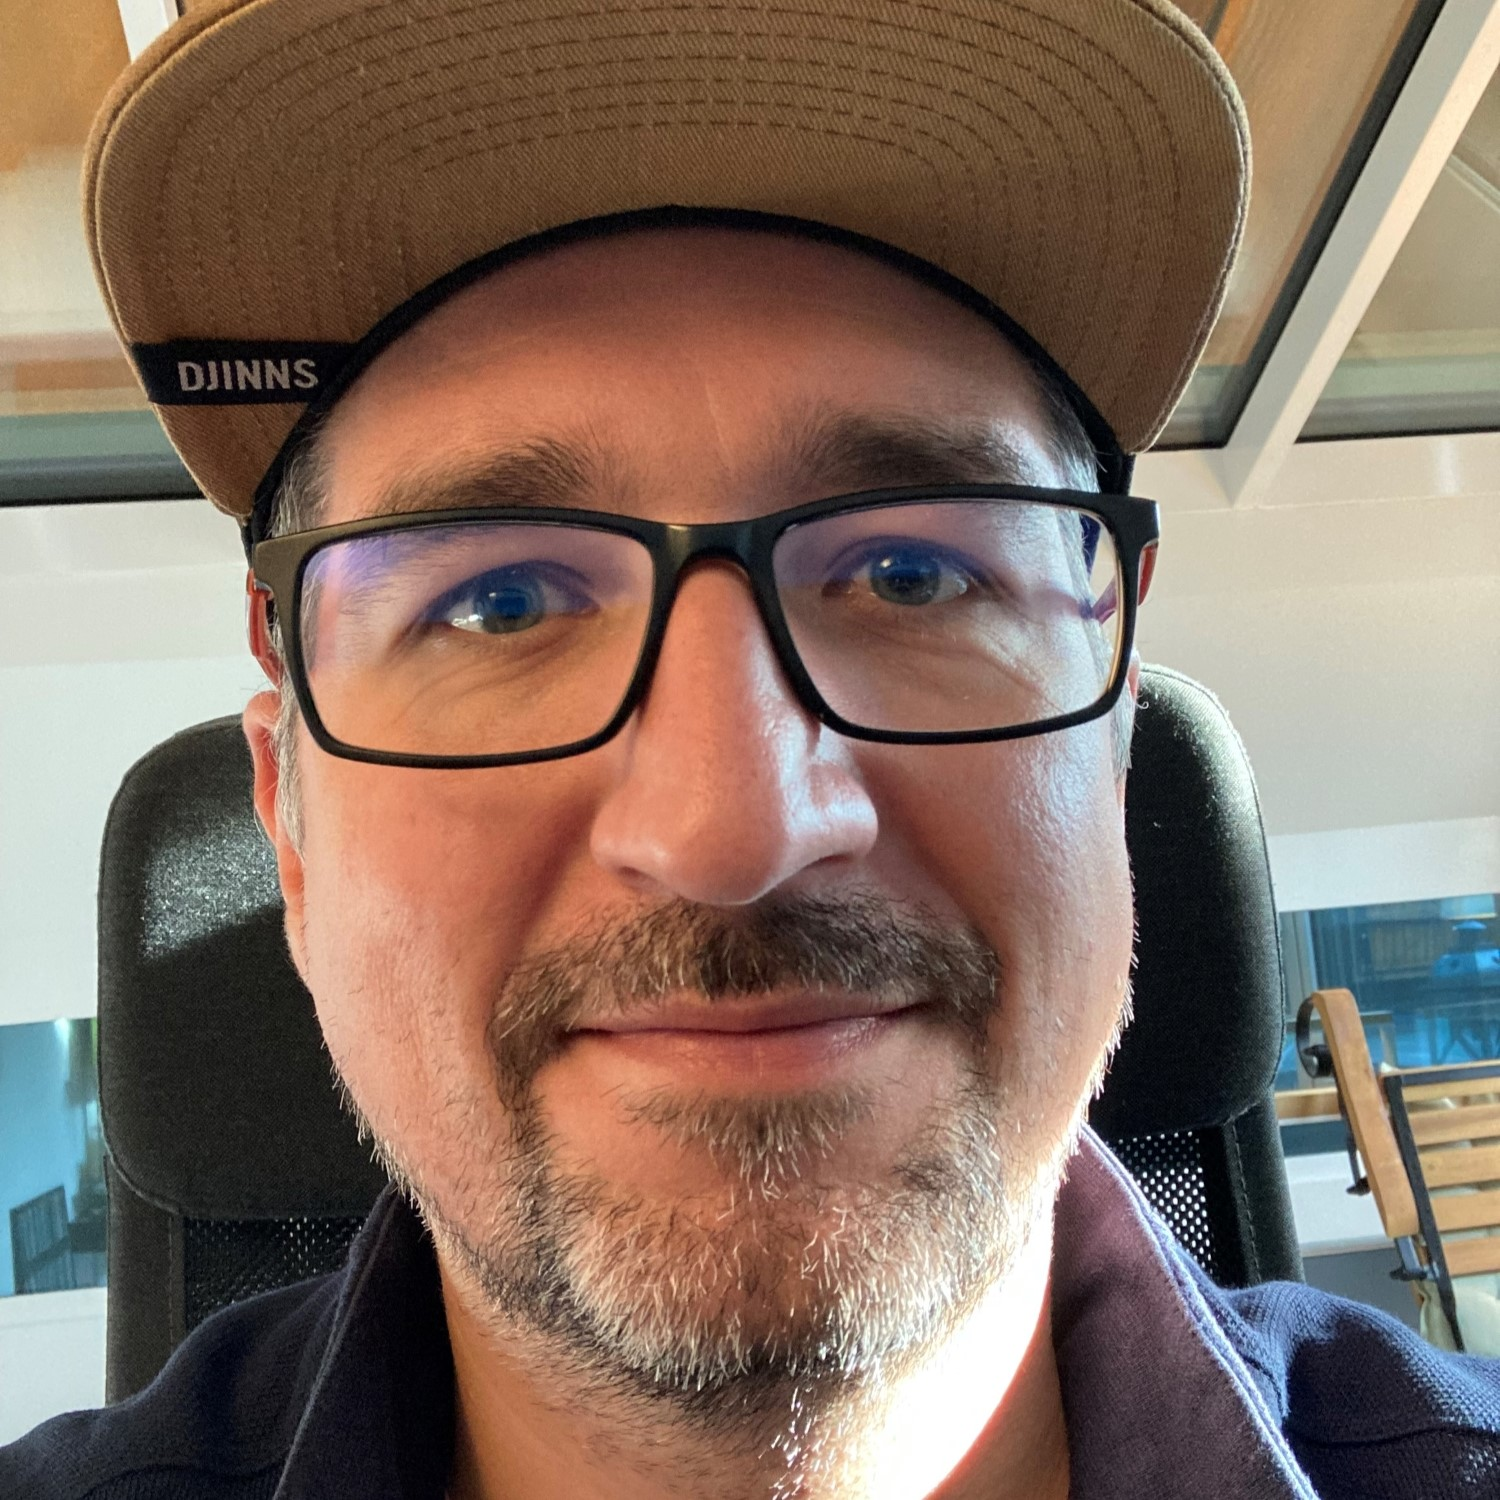
\includegraphics[width=0.8\textwidth]{schaermu_quad.jpg}
\end{minipage}
\hfill % Automatic horizontal whitespace

\vspace{0.75cm} % Vertical whitespace

\begin{minipage}[t]{1\textwidth} % Center column with the first column of icons
	\vspace{-\baselineskip} % Required for vertically aligning minipages

	% The first parameter is the FontAwesome icon name, the second is the box size and the third is the text
	% Other icons can be found by referring to fontawesome5.pdf (supplied with the template) and using the word after \fa in the command for the icon you want
	\icon{At}{12}schaermu@pm.me\hspace{0.2cm}
	\icon{Globe}{12}schaermu.ch/cv\hspace{0.2cm}
	\icon{Github}{12}github.com/schaermu\hspace{0.2cm}
\end{minipage}

\vspace{0.5cm} % Vertical whitespace

%----------------------------------------------------------------------------------------
%	INTRODUCTION, SKILLS AND TECHNOLOGIES
%----------------------------------------------------------------------------------------

\cvsect{Who am I?}

\begin{minipage}[t]{0.4\textwidth} % Left column with the introduction text, change the width as needed
	\vspace{-\baselineskip} % Required for vertically aligning minipages
	Ever since I meticulously typed the first BASIC scripts from the AMIGA magazine into my Amiga 600 in the 90s, I have been fascinated by software development and all its facets. The statement “Just turn your hobby into a profession” from the owner of a graphics studio was the catalyst for a multi-faceted career in information technology, which I am still as passionate about over 20 years later as I was on the first day.\\
\end{minipage}
\hfill % Automatic horizontal whitespace
\vspace{0.25cm} % Vertical whitespace
\begin{minipage}[t]{0.5\textwidth} % Right column with the skills bar chart, change the width as needed
	\vspace{-\baselineskip} % Required for vertically aligning minipages

	\begin{barchart}{5.5} % The parameter to the barchart environment is the maximum width (in cm) of the longest bar}
		\baritem{CI/CD}{90}
		\baritem{Git}{90}
		\baritem{Backend-Dev}{80}
		\baritem{Container}{70}
		\baritem{Linux/Shell}{60}
		\baritem{Cloud (AWS)}{60}
		\baritem{Monitoring}{40}
	\end{barchart}
\end{minipage}

% Output a series of bubbles showing your proficiency with environments and/or tools
\begin{center}
	\bubbles{4/GitLab, 5/GitHub, 4/Go, 6/VS Code, 5/Git, 5/TypeScript, 5/AWS, 5/Python} % Each bubble must be in the format of '<size>/<label>' and you can specify as many bubbles as will fit on the page
\end{center}

%----------------------------------------------------------------------------------------
%	EXPERIENCE
%----------------------------------------------------------------------------------------

\cvsect{Work experience}

\begin{entrylist}
	\entry
	{\footnotesize 10/2022 -- today}
	{Requirements-to-Deployment Manager}
	{Post CH AG}
	{As a Requirements-to-Deployment Manager, I am responsible for the technical leadership for 13 teams in the domain of software development and support them in all aspects related to software engineering as a coach and mentor. This can cover a wide range of areas, such as requirements engineering, ways of working, methodology, standard tools \& developer experience or CI/CD \& automation. Where necessary, I also assist teams with implementation, for example when migrating to new CI/CD platforms, adopting new process models or when planning \& budgeting technological lifecycles.\\ \\
		In close cooperation with my management team, I also drive the strategic development of the department. This includes establishing various tools for strategy implementation such as OKR, flight levels, portfolio management and reporting dashboards.\\ \\
		As a Cloud Portfolio Owner, I am also responsible for driving forward the Group-wide Post2Cloud project within our department and support the teams in planning and implementing the migration to modern cloud technologies and platforms.\\ \\ \small \texttt{CI/CD}\slashsep\texttt{SAFe \& Scrum}\slashsep\texttt{Cloud}\slashsep\texttt{Way-of-Work}\slashsep\texttt{Strategy \& OKR}\slashsep\texttt{Leadership}}
	\entry
	{\footnotesize 11/2018 -- 10/2022}
	{Full-Stack Developer}
	{Post CH AG}
	{As part of a small, high-performing team, I was tasked with developing various proof-of-concepts and market-ready MVPs for our business departments using a wide range of web, augmented reality, voice and AI technologies. A strong focus was placed on design thinking approaches with the relevant stakeholders to maximize impact within the shortest possible time to quickly test ideas on the market. I was also responsible for setting up an internal, cloud-based platform for innovation projects and was involved in various internal innovation initiatives and working groups.\\ \\From 2020 to 2022, I acted as co-lead for the design and rollout of a security champion program within the IT development department.\\ \\ \small \texttt{Prototyping}\slashsep\texttt{Security}\slashsep\texttt{Terraform}\slashsep\texttt{dotnet Core}\slashsep\texttt{Postgres}\slashsep\texttt{Angular}\slashsep\texttt{Cloud-Engineering}\slashsep\texttt{Scrum/Kanban}\slashsep\texttt{Design Thinking}\slashsep\texttt{Innovation}}
	\entry
	{\footnotesize 10/2016 -- 10/2018}
	{Full-Stack Developer}
	{smartfactory GmbH}
	{As part of a small, multi-national team consisting of both App- and Backend-Developers, I was entrusted with the realization of various client projects. Most of these were implemented with Django-based API's and Vue.js or Ionic-based frontends.\\ \\ In addition to the project business, I actively drove and successfully implemented the modernization of the CI/CD platform on GitLab as well as the automation of all release and deployment processes with Ansible.\\ \\ \small \texttt{Django}\slashsep\texttt{Laravel}\slashsep\texttt{Angular}\slashsep\texttt{Linux}\slashsep\texttt{Ansible}\slashsep\texttt{CI/CD}\slashsep\texttt{Scrum}\slashsep\texttt{GitLab}}

	\entry
	{\footnotesize 06/2012 -- 05/2016}
	{Software-Developer / Teamlead}
	{Maxomedia AG}
	{As a member of a software team, I accompanied the agile implementation of various client projects together with colleagues from the agency's creative department, including national campaigns for SBB, Postfinance and PostBus. I was also heavily involved in the modernization of the CI/CD pipeline and agile working methods. From the beginning of 2015, I was able to be team lead for a team of 4 developers as well as taking on technical responsibility for the internal CI/CD infrastructure and processes.\\ \\ \small \texttt{dotnet Core}\slashsep\texttt{node.js}\slashsep\texttt{MSSQL Server}\slashsep\texttt{CI/CD}\slashsep\texttt{Leadership}\slashsep\texttt{Scrum}}

	\entry
	{\footnotesize 10/2003 -- 05/2012}
	{Web-Developer}
	{various Companies}
	{During the time after my apprenticeship, I was privileged to implement and support custom software solutions in different companies for clients such as Kuoni, Migros, Hotelplan and the banking sector. The subject of CI/CD was present at each of these stations, in many different ways: in some places it was about building these processes from scratch, in other environments it was about evolving and modernizing them. In terms of technology, I mainly worked with Dotnet, PHP, node.js, MySQL and MSSQL with a strong emphasis on backend development.\\ \\ \small \texttt{Dotnet}\slashsep\texttt{PHP}\slashsep\texttt{node.js}\slashsep\texttt{Linux}\slashsep\texttt{Apache/IIS}\slashsep\texttt{Server-Maintenance}\slashsep\texttt{CI/CD}}

\end{entrylist}

%----------------------------------------------------------------------------------------
%	EDUCATION
%----------------------------------------------------------------------------------------

\vspace{0.5cm} % Vertical whitespace
\cvsect{Education}

\begin{entrylist}
	\entry
	{\footnotesize 08/1999 -- 09/2003}
	{Computer Scientist EFZ}
	{SBB CH AG}
	{Trained as a computer scientist at SBB CH AG (from 2002 at login Berufsbildung AG) specializing in software development. I conducted my final thesis in the field of web development in PHP.}
\end{entrylist}

%----------------------------------------------------------------------------------------
%	ADDITIONAL INFORMATION
%----------------------------------------------------------------------------------------

\vspace{0.5cm} % Vertical whitespace
\begin{minipage}[t]{0.45\textwidth} % Left column width
	\vspace{-\baselineskip} % Required for vertically aligning minipages

	\cvsect{Languages}

	\textbf{German} -- Native language\\
	\textbf{English} -- C1\\
	\textbf{French} -- A1/A2
\end{minipage}
\hfill % Automatic horizontal whitespace
\begin{minipage}[t]{0.45\textwidth} % Center column width
	\vspace{-\baselineskip} % Required for vertically aligning minipages

	\cvsect{References}

	upon request
\end{minipage}

%----------------------------------------------------------------------------------------

\end{document}
